\documentclass[12pt]{article}
%\documentclass{article}

\usepackage{amsmath,amsthm,amssymb,xcolor,graphicx,tikz}
\usepackage[pdftex]{hyperref}
\usetikzlibrary{positioning}

\begin{document}

\def\imp{\Rightarrow}
\def\true{\text{true}}
\def\false{\text{false}}
\def\pair{\text{pair}}
\def\fst{\text{fst}}
\def\snd{\text{snd}}
\def\succ{\text{succ}}
\def\pred{\text{pred}}
\def\self{\text{self}}
\def\Prexp{\text{Pr}_{\text{exp}}}

\newcommand{\goedel}[1]{\ulcorner #1 \urcorner}
\newcommand{\rstar}[1]{#1^*}
\newcommand{\rplus}[1]{#1^+}
\newcommand{\reqv}[1]{#1^\sim}
\newcommand{\toplus}{\rplus\to}
\newcommand{\tostar}{\rstar\to}
\newcommand{\tobeta}{\to_\beta}
\newcommand{\tobetaplus}{\to^+_\beta}
\newcommand{\tobetastar}{\to^*_\beta}
\newcommand{\tobetap}{\to_{p}}
\newcommand{\tobetapplus}{\to^+_{p}}
\newcommand{\tobetapstar}{\to^*_{p}}
\newcommand{\betaeqv}{\sim_\beta}
\newcommand{\toeqv}{\reqv\to}
\newcommand{\neglow}{\neg\,}
\newcommand{\lambdaw}{\lambda\,}
\newcommand{\upshift}{{\uparrow}}

\newcommand{\diamg}[6]{
  \begin{matrix}
    #3 & #1 & #4 \\
    #2 &      & #2 \\
    #5 & #1 & #6
  \end{matrix}
}
\newcommand{\diam} [4] {
  \diamg{\to}{\downarrow}{#1}{#2}{#3}{#4}
}
\newcommand{\diamp} [4] {
  \diamg{\to_p}{\downarrow_p}{#1}{#2}{#3}{#4}
}

\newcommand{\indrule}[2]{\begin{array}{l} #1 \\ \hline #2\end{array}}
\newcommand{\ruleh}[2]{\begin{array}{c} #1 \\ \hline #2\end{array}}
\newcommand{\rulev}[2]{\begin{array}{l} #1 \\ \hline #2\end{array}}

\theoremstyle{definition} \newtheorem{definition}{Definition}[section]
\theoremstyle{definition} \newtheorem{theorem}[definition]{Theorem}
\theoremstyle{definition} \newtheorem{lemma}[definition]{Lemma}


\title{Lambda Calculus - Step by Step}
\author{Helmut Brandl \\ \scriptsize (firstname dot lastname at gmx dot net)}
\date{}

\maketitle

\abstract{

  This little text gives a step by step introduction into untyped lambda
  calculus. All needed theory is explained and no special know how is
  assumed. Although elementary, all important theorems about untyped lambda
  calculus including some undecidability theorems are given and proved within
  this text.

  It has been tried to use a notation which is easy to understand with a lot
  of graphic notation to support a good intuition about the presented
  material.  }


\tableofcontents


\section{Motivation}

Why study lambda calculus?

Let us put the question in some historical context. At the beginning of the
20th century the famous mathematician David Hilbert challenged the
mathematical community by the statement that mathematical problems must be
decidable. At the 1930 annual meeting of the \emph{Society of German
  Scientists and Physicians} he made his famous quote ``We must know, we will
know''.

\noindent
\begin{tikzpicture}[scale=0.70]
  \def\pict#1#2#3#4{
    \node[fill=gray!20,text width=3.5cm,text centered] (#1) at #2
    {\scriptsize \includegraphics[width=3cm,height=4cm]{#3} #4};
  }
  \pict{hilbert}{(0,7)}{hilbert.jpg}{David Hilbert}

  \node[draw,fill=gray!30,text width=6cm] (text) at (10,8) {``Entscheidungsproblem''
    (Decision Problem). Mathematics must be decidable. ``We must know, we will
    know!''};

  \pict{goedel}{(0,0)}{goedel.jpg}{Kurt Gödel~(1931): Incompleteness Theorems}
  \pict{church}{(6,0)}{church.jpg}{Alonzo~Church~(1936): Lambda Calculus}
  \pict{turing}{(12,0)}{turing.jpg}{Alan Turing~(1936): Turing Machine}

  \draw [thick,->] (hilbert) -- (text) node[above,midway,sloped]{Challenge};
\end{tikzpicture}


The young mathematician Kurt Gödel attended the meeting and expressed some
doubts to his collegues about the general decidability of mathematical
statements. One year later in 1931 he published his famous incompleteness
theorems~\cite{goedel1931}. He proved that for all consistent formal systems
which are capable of expressing logic and doing simple arithmetics there are
certain statements which are not provable withing the system but true. These
incompleteness theorems are considered as the first serious blow of Hilbert's
program.

Five years later Alonzo Church~\cite{church1936} and Alan
Turing~\cite{turing1936} independently proved that the \emph{decision problem}
cannot be solved. Alonzo Church invented the lambda calculus and Alan Turing
his automatic machine (today called Turing machine) which are both equivalent
in expressiveness.

Although Church's lambda calculus has been published slightly before Alan
Turing published his paper on automatic machines usually Turing machines are
used define computability and decidability. Turing machines resemble more the
structure of modern computers than lambda calculus. A programming language is
called \emph{Turing complete} if all possible algorithms can be coded within
the language. Nobody talks about \emph{lambda complete}.

However lambda calculus is a quite fascinating model of computation.  The
lambda calculus invented by Alonzo Church is remarkably simple. It consists
just of variables, function applications and lambda abstractions. But the
calculus is sufficiently powerful to express all computable functions and
decision procedures.

Beside its expressive power lambda calculus is used as the theoretical base of
functional languages like Haskell, ML, F\#.

In this paper we explain the lambda calculus in its purest form as untyped
lambda calculus.

%%% Local Variables:
%%% mode: latex
%%% TeX-master: "main_untyped_lambda"
%%% End:


\section{Inductive Sets and Relations}
\label{setrelation}

\subsection{Inductive Sets}

\paragraph{Set Notation}

A set is an unordered collection of objects. If the object $a$ is an element of the set
$A$ we write $a \in A$.

A set $A$ is a subset of set $B$ if all elements of the set $A$ are also
elements of the set $B$. The symbol $\subseteq$ is used to express the subset
relation. The operator $:=$ is used to express that something is valid by
definition. Therefore the subset relation is defined symbolically by
$A \subseteq B := \forall a\mathbin. a \in A \imp a \in B$. The statement
$A \subseteq B$ can always be replaced by its definition
$\forall a\mathbin. a \in A \imp a \in B$ and vice versa.

The double arrow $\imp$ is used to express implication. $p \imp q$ states the
assertion that having a proof of $p$ we can conclude $q$. The assertion $p
\imp q$ is proved by assuming $p$ and deriving the validity of $q$.




\paragraph{Rule Notation}

We have often several premises which are needed reach a conclusion. E.g. we
might have the assertion $p_1 \land p_2 \land \ldots \imp c$. Then we use the
rule notation $\ruleh{p_1, p_2, \ldots}{c}$ or $\rulev{p_1 \\ p_2\\
  \vdots}{c}$ to express the same fact. Evidently the order of the premises is
not important.

Variable in rules are universally quantified. Therefore we can state the
subset definition $\forall a\mathbin. a \in A \imp a \in B$. in rule notation more
compactly and better readable as $\ruleh{a \in A}{a \in B}$. It should be clear
from the context which symbols denote variables.


\paragraph{Inductive Definition of Sets}

Rules can be used to define sets inductively. The set of even numbers $E$ can be
defined by the two rules $0 \in E$ and $\ruleh {n \in E}{n+2 \in E}$. A set
defined by rules is the least set which satisfies the rules. The set $E$ of
even number must contain the number $0$ and with all numbers $n$ it contains
also the number $n+2$.

The fact that some object is an element of an inductively defined set must be
established by an arbitrarily long but finite sequence of applications of the
rules which define the set. A proof of $4 \in E$ consists of a proof of $0 \in
E$ by application of the first rule and then two applications of the second
rule to reach $2 \in E$ and $4 \in E$.






\paragraph{Rule Induction}

If we have the fact that an object is an element of some inductively defined
set then we can be sure that it is in the set because of one of the rules
which define the set.

This can be used to prove facts by rule induction. Suppose we want to prove
that some property $p$ is shared by all even numbers. We can express this
statement by the rule $\ruleh {n \in E}{p(n)}$. Note that variables in rules
are implicitly universally quantified, i.e. the rule expresses the statement
$\forall n \mathbin. n \in E \imp p(n)$.

It is possible to prove this statement by induction on $n \in E$. Such a proof
consists of a proof of the statement for each rule. In the case of even
numbers there are two rules.

For the first rule we have to prove the the number $0$ satisfies the property
$p(0)$.

For the second rule we assume that $n \in E$ because there is some other
number $m$ already in the set of even numbers $E$ and $n = m+2$. I.e. we have
to prove the goal $p(m+2)$ under the premise $m \in E$. Because of the premise
$m \in E$ we can assume the induction hypothesis $p(m)$. I.e. we can assume
$m \in E$ and $p(m)$ and derive the validity of $p(m+2)$.

If the proof succeeds for both rules we are allowed to conclude that the
property $p$ is satisfied by all even numbers.



\paragraph{Natural Number Induction}

It is not difficult to see that the usual law of induction on natural numbers
is just a special case of rule induction. We can define the set of natural
numbers inductively $\mathbb{N}$ by the rules
\begin{enumerate}
\item $0 \in \mathbb{N}$
\item $\ruleh{n \in \mathbb{N}} {n' \in \mathbb{N}}$
\end{enumerate}
where $n'$ denotes the successor of $n$ i.e. $3$ is just a shorthand for
$0'''$.

The usual induction law of natural numbers allows to prove a property $p$ for
all natural number by a proof of $p(0)$ and a proof of
$\forall n\mathbin. p(n) \imp p(n')$ which are exactly the requirements of a
proof by rule induction.





\paragraph{Grammar Notation}

In some cases it is convenient to define a set by a grammar. E.g. we can
define the set of natural numbers by all terms $n$ generated by the grammar
%
    $$ n ::= 0 \mid n'$$
%
i.e. we can use the corresponding induction law to prove
that all terms generated by the grammar satisfy a certain property.

This definition is just a special form of the definition of the set of natural
numbers $\mathbb{N}$ by the rules
\begin{enumerate}
\item $0 \in \mathbb{N}$
\item $\ruleh{n \in \mathbb{N}} {n' \in \mathbb{N}}$
\end{enumerate}





\subsection{Inductive Relations}


\paragraph{Relations}

n-ary relations are just sets of n-tuples. A binary relation $r$ over the sets
$A$ and $B$ is a subset of the cartesian product
$$
    r \subseteq A \times B.
$$ We use the notations $(a,b) \in r$, $r(a,b)$ and $a \to_r b$ to denote the
fact that the pair $(a,b)$ with $a \in A$ and $b \in B$ figure in the relation
$r$.

In this paper we need only endorelations i.e. binary relations where the
domain $A$ and the range $B$ of the relation are the same set.




\paragraph{Relation Closure}

As with sets, relations can be defined inductively.


% Transitive Closure
% --------------
\begin{definition} The \emph{transitive closure} $\rplus{r}$ of a relation $r$ is
  defined by the rules
  \begin{enumerate}
  \item $\ruleh {r(a,b)} {\rplus{r}(a,b)}$
  \item $\ruleh{\rplus{r}(a,b),\, r(b,c)}{\rplus{r}(a,c)}$
  \end{enumerate}
\end{definition}

The rules can be displayed graphically. The premises are marked blue and the
conclusion is marked red.

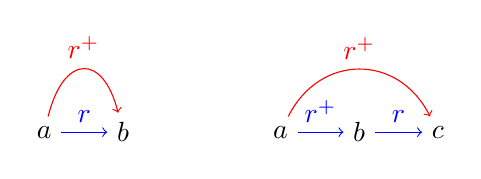
\begin{tikzpicture}
  \node (a0) at (0,0) {$a$};
  \node (b0) at (1,0) {$b$};

  \node (a) at (3,0) {$a$};
  \node (b) at (4,0) {$b$};
  \node (c) at (5,0) {$c$};

  \draw [->,blue] (a0) edge node[above]{$r$} (b0);
  \draw [->,red]   (a0) .. controls (0.25,1) and (0.75,1) .. node[above] {$r^+$} (b0);

  \path[->,blue] (a) edge node[above] {$r^+$} (b);
  \path[->,blue] (b) edge node[above] {$r$}    (c);
  \draw[->,red]   (a) .. controls (3.5,1) and (4.5,1) ..  node[above] {$r^+$}    (c);
\end{tikzpicture}


We called $r^+$ the transitive closure of $r$, but the fact that $r^+$ is
transitive needs a proof.

\begin{theorem}
  \label{plustransitive}
  The transitive closure $r^+$ of the relation $r$ is transitive
  i.e. $\ruleh{a \to_r^+ b, \, b \to_r^+ c} {a \to_r^+ c}$ is valid.
  \begin{proof}
    Assume $a \to_r^+ b$ and prove the goal $a \to_r^+ c$ by induction on
    $b \to_r^+ c$.
    \begin{enumerate}
    \item
      Goal $a \to_r^+ c$ assuming $b \to_r^+ c$ and that
      $b \to_r^+ c$ is valid by rule 1 of the transitive closure.\\
      Premise $b \to_r c$.\\
      The goal is valid by the assumption $a \to_r^+ b$, the premise $b \to_r
      c$ and rule 2 of the transitive closure.

    \item
      Goal $a \to_r^+d$ assuming $b \to_r^+ d$ and that
      $b \to_r^+ d$ is valid by rule 2 of the transitive closure. \\
      Premises $b \to_r^+ c$ and $c \to_r d$.\\
      Induction hypothesis $a \to_r^+ c$.\\
      The goal is valid by the induction hypothesis $a \to_r^+ c$, the premise
      $c \to_r d$ and rule 2 of the transitive closure.
    \end{enumerate}
  \end{proof}
\end{theorem}




% Reflexive Transitive Closure
% ----------------------
\begin{definition} The \emph{reflexive transitive closure} $\rstar{r}$ of a relation $r$ is
  defined by the rules
  \begin{enumerate}
  \item $\rstar{r}(a,a)$
  \item $\ruleh{\rstar{r}(a,b), \, r(b,c)}{\rstar{r}(a,c)}$
  \end{enumerate}
\end{definition}

Graphical representation of the rules:

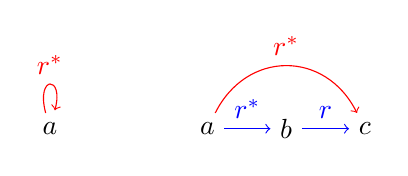
\begin{tikzpicture}
  \node (reflexive) at (0,0) {$a$};
  \node (a) at (2,0) {$a$};
  \node (b) at (3,0) {$b$};
  \node (c) at (4,0) {$c$};

  \path (reflexive) edge [loop above,red] node {$r^*$} (reflexive);

  \path[->,blue] (a) edge node[above] {$r^*$} (b);
  \path[->,blue] (b) edge node[above] {$r$}    (c);
  \draw[->,red]   (a) .. controls (2.5,1) and (3.5,1) ..  node[above] {$r^*$}    (c);
\end{tikzpicture}

\begin{theorem}
  \label{startranstive}
  The reflexive transitive closure $r^*$ of the relation $r$ is transitive
  i.e. $\ruleh{a \to_r^* b, \, b \to_r^* c} {a \to_r^* c}$ is valid.
  Proof similar to the proof of theorem~\ref{plustransitive}.
\end{theorem}




% Equivalence Closure
% ----------------
\begin{definition}
  \label{def:equivalenceclosure}
  The \emph{equivalence closure} $\reqv{r}$ of a relation $r$ is
  defined by the rules
  \begin{enumerate}
  \item
    $\reqv{r}(a,a)$
  \item
    $\ruleh{
      \reqv{r}(a,b), \,   r(b,c)}
    {\reqv{r}(a,c)}$
  \item
    $\ruleh{\reqv{r}(a,b), \, r(c,b)} {\reqv{r}(a,c)}$
  \end{enumerate}
\end{definition}

Again a graphical representation of the rules:

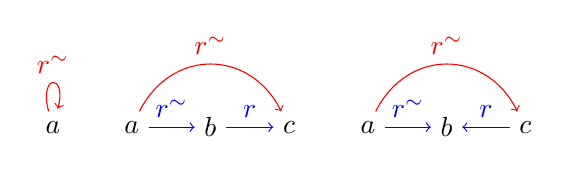
\begin{tikzpicture}
  \node (a0) at (0,0) {$a$};
  \path (a0) edge [loop above,red] node {$r^\sim$} (a0);

  \node (a1) at (1,0) {$a$};
  \node (b1) at (2,0) {$b$};
  \node (c1) at (3,0) {$c$};
  \draw[->,blue] (a1) edge node[above]{$r^\sim$} (b1);
  \draw[->,blue] (b1) edge node[above]{$r$} (c1);
  \draw[->,red] (a1) .. controls (1.5,1) and (2.5,1) .. node [above]{$r^\sim$} (c1);

  \node (a2) at (4,0) {$a$};
  \node (b2) at (5,0) {$b$};
  \node (c2) at (6,0) {$c$};
  \draw[->,blue] (a2) edge node[above]{$r^\sim$} (b2);
  \draw[<-,blue] (b2) edge node[above]{$r$} (c2);
  \draw[->,red]   (a2) .. controls (4.5,1) and (5.5,1) .. node [above]{$r^\sim$} (c2);
\end{tikzpicture}

\begin{theorem}
  \label{eqvtransitive}
  The equivalence closure is transitive. Proof similar to the proof of
  theorem~\ref{plustransitive}.
\end{theorem}

\begin{theorem}
  The equivalence closure is symmetric i.e. $\ruleh {a \to_r^\sim b} {b
    \to_r^\sim a}$.
  \begin{proof}
    We proof this theorem in 3 steps. First we proof two lemmas and then the
    theorem by induction.
    \begin{itemize}
    \item Lemma 1: $\ruleh{a \to_r b}{a \to_r^\sim b}$. Proof. Assume $a \to_r
      b$. We get $a \to_r^\sim a$ by rule 1 and then $a \to_r^\sim b$ by the
      assumption and rule 2.
    \item
      Lemma 2: $\ruleh{a \to_r b}{b \to_r^\sim a}$. Proof. Assume $a \to_r b$.
      We get $b \to_r^\sim b$ by rule 1 and then $b \to_r^\sim a$ by the
      assumption and rule 3.
    \item
      $\ruleh {a \to_r^\sim b} {b \to_r^\sim a}$ by induction on
      $a \to_r^\sim b$.
      \begin{enumerate}
      \item
        Goal $a \to_r^\sim a$. Trivial by reflexivity.

      \item
        Goal $c \to_r^\sim a$ assuming that $a \to_r^\sim c$ is valid by rule 2 of
        the equivalence closure.\\
        Premises $a\to_r^\sim b$ and $b \to_r c$.\\
        Induction hypothesis $b \to_r^\sim a$.\\
        We get $c \to_r^\sim b$ by the second premise and lemma 2 and then $c
        \to_r^\sim a$ by the induction hypothesis and transitivity of the
        equivalence closure~\ref{eqvtransitive}.

      \item
        Goal $c \to_r^\sim a$ assuming that $a \to_r^\sim c$ is valid by rule 3 of
        the equivalence closure.\\
        Premises $a\to_r^\sim b$ and $c \to_r b$.\\
        Induction hypothesis $b \to_r^\sim a$.\\
        We get $c \to_r^\sim b$ by the second premise and lemma 1 and then $c
        \to_r^\sim a$ by the induction hypothesis and transitivity of the
        equivalence closure~\ref{eqvtransitive}.

      \end{enumerate}
    \end{itemize}
  \end{proof}
\end{theorem}



% Closures are increasing, monotonic and idempotent
% -----------------------------------------
\begin{theorem}
  All closures are increasing $r \subseteq r^c$, monotonic
  $r \subseteq s \imp r^c \subseteq s^c$ and idempotent $r^{cc} = r^c$ (where
  the superscript $c$ stands for $+$, $*$ or $\sim$).
  \begin{proof}  We give a proof for the reflexive transitive closure. The
    proofs for the other closures are similar.
    \begin{itemize}
    \item
      Increasing: Goal $r(a,b) \imp \rstar{r}(a,b)$. By rule 1 we get
      $\rstar{r}(a,a)$. The assumption $r(a,b)$ and rule 2 imply
      $\rstar{r}(a,b)$.
      %
    \item
      Monotonic: Goal $\ruleh{r \subseteq s, \, \rstar{r}(a,b)}
      {\rstar{s}(a,b)}$. Prove by induction on $\rstar{r}(a,b)$.
        \begin{enumerate}
        \item Case $a=b$. Goal $s^*(a,a)$. Trivial by reflexivity of $\rstar{s}$.
        \item
          Goal $s^*(a,c)$ assuming $r\subseteq s$ and $r^*(a,c)$ is valid
          because of rule 2. Premises $r^*(a,b)$ and $r(b,c)$. Induction
          hypothesis $s^*(a,b)$.
          \\
          $
          \begin{matrix}
            a  & \to_{\rstar{r}} & b   &  \to_r   & c \\
                &    \Downarrow_1 & &  \Downarrow_2\\
            a  & \to_{\rstar{s}} & b   &  \to_s  &  c
          \end{matrix}$.\\
          $\Downarrow_1$ is valid by the induction
          hypothesis. $\Downarrow_2$ is valid by $r \subseteq s$. From the
          last line and the rule 2 of the reflexive transitive closure we can
          conclude $\rstar{s}(a,c)$.
        \end{enumerate}
    \item
      Idempotent: The equality of the relations $r^{**} = r^*$ needs a proof
      of $r^{**} \subseteq r^*$ and a proof of $r^* \subseteq r^{**}$.
      \begin{itemize}
      \item $ r^* \subseteq r^{**}$ is valid because the
        closure is increasing.
      \item
        Goal $\ruleh{r^{**}(a,b)} {r^*(a,b)}$. Proof by induction on $r^{**}(a,b)$.
        \begin{enumerate}
        \item
          Case $a=b$. Goal $r^*(a,a)$. Trivial by reflexivity.
        \item
          Goal $r^*(a,c)$ assuming $r^{**}(a,c)$ is valid because of rule 2.
          Premises $r^{**}(a,b)$ and $r^*(b,c)$. Induction
          hypothesis $r^*(a,b)$.
          $
          \begin{matrix}
            a  & \to_{r^{**}} & b   &  \to_{r^*}   & c \\
                &    \Downarrow_1 & &  \Downarrow_2\\
            a  & \to_{r^*} & b   &     \to_{r^*}   &  c
          \end{matrix}$.
          $\Downarrow_1$ is valid by the induction
          hypothesis. $\Downarrow_2$ is trivial. $r^*$ is
          transitive. Therefore the last line implies $r^*(a,c)$.
        \end{enumerate}
      \end{itemize}
    \end{itemize}
  \end{proof}
\end{theorem}






\begin{theorem}
  \label{sameclosure}
A relation $s$ which satisfies $r \subseteq s \subseteq r^c$ has the same closure
as $r$ i.e. $r^c = s^c$. Proof:
  \begin{itemize}
  \item $r^c \subseteq s^c$ by monotonicity.
  \item $s^c \subseteq r^c$: $s^c \subseteq r^{cc}$ by
    monotonicity and then use idempotence to conclude $s^c \subseteq r^c$.
  \end{itemize}
\end{theorem}





\paragraph{Terminal Elements}

\begin{definition}
  The set of \emph{terminal elements} $T_r$ of the relation $r$ is
  defined by the rule
  $$
  \ruleh{
    \begin{bmatrix}
      \ruleh {a\to b} {\perp}
    \end{bmatrix}}
  {a \in T_r}$$
%
  where $\perp$ is used to denote a contradiction and the square brackets $[$
  and $]$ around the rule above the line indicate that the variables not used
  outside the bracketed rule are universally quantified in the inner
  rule. I.e. in order to establish $a \in T_r$ we have to prove
  $\forall b \mathbin. \neglow (a \to_r b)$ or
  $\forall b\mathbin. a \to_r b \imp \perp$.
%
  Note that the scope of the universal quantification of the variable $a$
  spans the whole rule while the scope of the universal quantification of the
  variable $b$ is just the premise of the rule (i.e. the part above the line).
\end{definition}



\begin{theorem}
  \label{trivialpaths}
  A terminal element $a$ of a relation $r$ has only trivial outgoing paths:
  $\ruleh {a \in T_r, \, a \to_r^* b} {a = b}$.
  \begin{proof} By induction on $a \to_r^* b$.
    \begin{enumerate}
    \item
      Goal $a = a$. Trivial.
    \item
      Goal $a = c$ assuming that $a \to_r^* c$ is valid by rule 2. Premises
      $r^*(a,b)$ and $r(b,c)$. Induction hypothesis $a = b$. Therefore the
      second premise states $r(a,c)$ which contradicts the assumption $a \in T_r$.
    \end{enumerate}
  \end{proof}
\end{theorem}




\paragraph{Weakly Terminating Elements}

\begin{definition}
  $a$ is a \emph{(weakly) terminating element} of the relation $r$ if there
  is a path to a terminal element $b$ i.e. $a \to_r^* b$. The set of
  \emph{weakly terminating elements} $WT_r$ of the relation $r$ is defined by
  the rule $\ruleh{a \to_r^* b, \, b \in T_r} {a \in WT_r}$.
\end{definition}






\paragraph{Strongly Terminating Elements}

\begin{definition}
  An object $a$ is \emph{strongly terminating} with respect to the relation
  $r$ if all paths from $a$ end at some terminal element of $r$. We define the
  set of strongly terminating elements $ST_r$ of the relation $r$ by the rule
%
$$
   \ruleh
   {
     \begin{bmatrix}
       \ruleh {a \to_r b} {b \in ST_r}
     \end{bmatrix}
   }
   {a \in ST_r}
$$
\end{definition}

This definition might need some explanation to be understood correctly. Since
the premise of the rule is within brackets, all variables not occuring outside
the brackets are universally quantified within the brackets (here the variable
$b$).

The rule says that all objects $a$ where all successors $b$ with respect to
the relation are strongly terminating are strongly terminating as well. The
rule is trivially satisfied by all objects which have no successors i.e. all
terminal objects. If the relation $r$ has no terminal objects then there
are no initial objects which are strongly terminating.

If there are terminal elements then step by step strongly terminating objects
can be constructed by the rule that all successors of them must be strongly
terminating (or already terminal). For each constructed strongly terminating
object it is guaranteed that all paths starting from it must end within a finite
number of steps at some terminal object of the relation.




An object $a$ without successors with respect to the relation $r$ i.e. if
there are no $b$ with $a \to_r b$ satisfy the rule, because the premise is
satified vacuously. An object $a$ without successors is a terminal element by
definition. I.e. all terminal elements are strongly terminating.










\subsection{Diamonds and Confluence}
\label{sec:diamondsconfluence}

In this section we define diamonds and confluent relations.

A relation is called confluent if starting from some object following the
relation on different paths of arbitrary length there is always some other
object where the two paths meet. This intuitive definition is made precise in
the following.

A diamond relation is a kind of a confluent relation where one step different
paths can join withing one step.

It turns out that confluence is a rather strong property of a relation. It
guarantees that
\begin{itemize}
\item all equivalent elements meet at some point
\item all paths to terminal elements end up at the same terminal
  element (i.e. terminal elements are unique)
\end{itemize}

A diamond relation is a superset of a confluent relation which has already the
essential part of confluence. It turns out that a diamond relation is confluent.

First we define formally the diamond property of a relation. The diamond
property is intuitively a one step confluence.

\begin{definition}
A relation $r$ is a \emph{diamond} if for all $a$, $b$ and $c$ there exists a $d$
such that
$
  \begin{matrix}
    a & \to_r & b \\
    \downarrow_r & & \downarrow_r \\
    c & \to_r & \exists d
  \end{matrix}
$ holds.
\end{definition}

\noindent Note that we use the picture
$$\begin{matrix}
  a & \to_r & b \\
  \downarrow_r & & \downarrow_r \\
  c & \to_r & \exists d
\end{matrix}$$ to express the statement
$$\ruleh {a \to_r b, \, a \to_r c} {\exists d\mathbin. b\to_r d \land c\to_r
  d}.$$
%
The picture notation is more intuitive but not less precise because it can be
translated into the corresponding rule notation which can be translated
uniquely into a statement of predicate logic.

\begin{definition}
  A relation $r$ is \emph{confluent} if $\rstar{r}$ is a diamond.
\end{definition}

\begin{theorem} In a confluent relation $r$ all two $r$-equivalent elements
  meet at some common element in zero or more steps
  $
  \begin{matrix}
    a & \to_r^\sim & b \\
    & \searrow_r^* & \downarrow_r^*\\
    & & \exists c
  \end{matrix}
  $.
  \begin{proof}
    By induction on $a \to_r^\sim b$.
    \begin{enumerate}

    \item $a = b$. Trivial. Take $c = a$.

    \item
      Goal
      $\begin{matrix}
        a    & \to_r^\sim      & c                      \\
              & \searrow_r^* & \downarrow_r^*  \\
        & & \exists e
      \end{matrix}$
      where $a \to_r^\sim c$ is valid by rule 2. Premises $a \to_r^\sim b$
      and $b \to_r c$.
      Induction hypothesis
      $\begin{matrix}
        a    & \to_r^\sim      & b                      \\
              & \searrow_r^* & \downarrow_*  \\
        & & \exists d
      \end{matrix}$.\\
      Proof
      $\begin{matrix}
        a & \reqv\to_r & b & \to_r & c\\
        & \searrow_r^* & \downarrow_r^*  & & \downarrow_r^*\\
        & & \exists d & \to_r^* & \exists e
      \end{matrix}$.
      $d$ exists by induction hypothesis, $e$ exists by confluence.

    \item
      Goal
      $\begin{matrix}
        a    & \to_r^\sim      & c                      \\
              & \searrow_r^* & \downarrow_r^*  \\
        & & \exists e
      \end{matrix}$
      where $a \to_r^\sim c$ is valid by rule 3. Premises $a \to_r^\sim b$
      and $b \gets_r c$.
      Induction hypothesis
      $\begin{matrix}
        a    & \to_r^\sim      & b                      \\
              & \searrow_r^* & \downarrow_r^*  \\
        & & \exists d
      \end{matrix}$.\\
      Proof
      $\begin{matrix}
        a              & \reqv\to_r       & b            & \gets_r & c \\
        & \searrow_r^* & \downarrow_r^* & \swarrow_r^* \\
        &              & \exists d
      \end{matrix}$.
      $d$ exists by induction hypothesis.
    \end{enumerate}
  \end{proof}
\end{theorem}


\begin{theorem}
  In a confluent relation all paths from the same object ending at some terminal
  object end at the same terminal object, i.e.
  $$\ruleh {a \to_r^* b, \, a \to_r^* c, \, b \in T_r, \, c \in T_r} {b = c}$$.

  \begin{proof}
    Suppose there are two terminal elements $b$ and $c$ with paths starting
    from the object $a$.
    By definition of confluence there must be a $d$ such that
    $\begin{matrix} a & \to_r^* & b \\
      \downarrow_r^* & & \downarrow_r^* \\
      c & \to_r^* & d
    \end{matrix}$ is valid. Since $b$ and $c$ are terminal objects by
    theorem~\ref{trivialpaths} there are only trivial outgoing paths from $b$
    and $c$ which implies that $b = c = d$ must be valid.
  \end{proof}
\end{theorem}


\begin{theorem}
  \label{th:diamondconfluent}
  A diamond relation is confluent.
  \begin{proof}
    We prove this theorem in two steps.
    \begin{itemize}
    \item Lemma: Let $r$ be a diamond. Then
      $\begin{matrix}
        a                     &    \to_r^*    &    b \\
        \downarrow_r &                   & \downarrow_r \\
        c                     & \to_r^*       & \exists d
      \end{matrix}$ is valid.
      Proof by induction on $a \to_r^* b$.
      \begin{enumerate}
      \item
        Case $a = b$. Trivial, take $d=c$.
      \item
        Goal $\begin{matrix}
          a                     &    \to_r^*    &    c \\
          \downarrow_r &                   & \downarrow_r \\
          d                     & \to_r^*       & \exists f
        \end{matrix}$ where $a \to_r^* c$ is valid because of rule 2.
        Premises $a \to_r^* b$ and $b \to_r c$.
        Induction hypothesis
        $\begin{matrix}
          a                     &    \to_r^*    &    b \\
          \downarrow_r &                   & \downarrow_r \\
          d                     & \to_r^*       & \exists e
        \end{matrix}$.
        \\
        Proof:
        $\begin{matrix}
          a                     & \to_r^* & b                     & \to_r & c\\
          \downarrow_r &             & \downarrow_r &          & \downarrow_r\\
          d                     & \to_r^* & \exists e        & \to_r & \exists f
        \end{matrix}$. $e$ exists by the induction hypothesis, $f$ exists because
        $\to_r$ is a diamond.
      \end{enumerate}

    \item Theorem:  Let $r$ be a diamond. Then
      $\begin{matrix}
        a                     & \to_r^*     & b \\
        \downarrow_r^* &                 & \downarrow_r^* \\
        c                        & \to_r^*     & \exists d
      \end{matrix}$ is valid.
      Proof by induction on $a \to_r^* c$.
      \begin{enumerate}
      \item
        Case $a = b$. Trivial, take $d=c$.
      \item
        Goal
        $\begin{matrix}
          a                     & \to_r^*     & b \\
          \downarrow_r^* &                 & \downarrow_r^* \\
          d                        & \to_r^*     & \exists f
        \end{matrix}$ where $a \to_r^* d$ is valid because of rule 2.
        Premises $a \to_r^* c$ and $c \to_r d$.
        Induction hypothesis
        $\begin{matrix}
          a                     & \to_r^*     & b \\
          \downarrow_r^* &                 & \downarrow_r^* \\
          c                        & \to_r^*     & \exists e
        \end{matrix}$.
        \\
        Proof
        $\begin{matrix}
          a                        & \to_r^*  & b\\
          \downarrow_r^* &              & \downarrow_r^* \\
          c                        & \to_r^*  & \exists e  \\
          \downarrow_r    &              & \downarrow_r \\
          d                        & \to_r^*  & \exists f
        \end{matrix}$.
        $e$ exists by induction hypothesis, $f$ exists by the previous lemma.
      \end{enumerate}
    \end{itemize}
  \end{proof}
\end{theorem}

The last theorem stating that diamonds are confluent gives a way to prove that
a relation $r$ is confluent. If $r$ is already a diamond we are ready since a
diamond is confluent. If $r$ is not a diamond we try to find a diamond
relation $s$ between $r$ and its reflexive transitive closure $r^*$ i.e. a
relation $s$ which satisfies $r \subseteq s \subseteq r^*$. From the
theorem~\ref{sameclosure} we know that $s$ and $r$ have the same reflexive
transitive closure i.e. $r^* = s^*$. Since $s$ is a diamond, $s^*$ is a
diamond as well and therefore $r$ is confluent.

In order to find a diamond relation $s$ we can search for rules which are
satisfied by $r^*$ and are intuitively the reason which let us assume that $r$
is confluent. Then we can define $s$ inductively as the least relation
satisfying the rules and hope that we can prove that $s$ is a diamond with $r
\subseteq s$. Note that $s \subseteq r^*$ is satisfied implicitly by this
approach since $r^*$ satisfies the rules and $s$ is the least relation
satisfying the rules.


\section{Lambda Terms}
\label{sec:lambda}

\subsection{Basic Definitions}

Imagine a mathematical function with one argument which triplicates the
argument and adds five to the result. How would you write such a function. In
mathematics the most straightforward notation is
$$ x \mapsto 3 \times x + 5.$$
%
The name of the variable $x$ is not important. We could write the same
function as $y \mapsto 3\times y + 5$. The variables $x$ and $y$ are called bound
variables because they are bound by the context definining the function.

Now suppose you want to apply the function to an actual argument, say
$2$. I.e. we want to compute $(x \mapsto 3\times x + 5)(2)$. We do it by
replacing the variable $x$ in the expression $3\times x + 5$ defining the
function by the argument $2$ resulting if $3\times 2 + 5$.

More formally we could write
$$ (x \mapsto 3 \times x + 5)(2) \to (3 \times x + 5)[x:=2] = 3\times 2 + 5.$$
where $\to$ means \emph{reduces to}.

That is already the essence of lambda calculus. In lambda calculus we write
the function $$x \mapsto 3 \times x + 5$$ as $$\lambda x. 3 \times x + 5.$$
and we write function application by juxtaposition
$$ (\lambda x. 3\times x + 5) 2$$
which reduces to
$$ (\lambda x. 3\times x + 5) 2 \to_\beta (3 \times x + 5)[x:=2]$$.
The application of the function to an argument is called a $\beta$-reduction.

$\beta$-reduction is done by variable substitution which can be done purely
mechanically i.e. it is the essence of a computation step.

In lambda calculus we have no primitive data types like booleans, numbers
pairs etc. There are only functions. However it is possible to represent data
by functions as we shall see later. Data are represented by functions which
capture the essence of what can be done by the data.

E.g. boolean values can be used to decide between two alternatives. Therefore
a boolean value is represented in lambda calculus by a function with two
arguments which chooses the first or second argument depending on its value.

Numbers are represented by functions which take two arguments, a function and
a start value and the lambda term representing the number iterates the
function n-times on the start value.



\paragraph{Definition of Lambda Terms}

\begin{definition}
  Let $x$ range over a countably infinite set of variable names
  $\{x_0, x_1, \ldots\}$ and $t$ over lambda terms, then the set of lambda
  terms is defined by the grammar $$t ::= x \mid t\, t \mid \lambda x. t.$$
\end{definition}

A lambda term is either a variable $x$, an application $a\,b$ (the term $a$
applied to the term $b$) or an abstraction $\lambda x.a$.

We use the convention that application is left associative i.e. $a b c$ is
parsed as $(a b) c$.

Nested lambda abstractions $\lambda x. \lambda y. \ldots . t$
are parsed as $\lambda x. (\lambda y. \ldots . t)$ and
abbreviated as $\lambda x y \ldots\, . t$.


\paragraph{Free and Bound Variables}

In the abstraction $$ \lambda x. t$$ the variable $x$ is a bound variable. It
is not visible to the outside world. This is the same convention as used in
programming languages which allow the definition of procedures. The formal
arguments names of the procedure/function arguments are just visible to the
definition of the procedure/function and not to the outside world.

Variables which are not bound by a lambda abstraction are free variables.

\begin{definition}
  The set of free variables $FV(t)$ of a lambda term $t$ is defined by
  $$FV(t) :=
  \begin{cases} FV(x) &= \{x\} \\
     FV(a b) &= FV(a) \cup FV(b) \\
     FV(\lambda x. t) &= FV(t) - \{x\}
   \end{cases}
   $$
\end{definition}

\begin{definition}
  A lambda term without free variables is called a \emph{closed lambda term}.
\end{definition}

Evidently bound variables can be renamed without changing the meaning of the
term. E.g. the two lamda terms
$$\lambda x. x $$
$$\lambda y. y  $$
are considered as the same term which represents the identity
function. Traditionally the terms are called $\alpha$-equivalent because you
transform one into the other by just renaming bound variables.

We write $t = u$ only if $u$ and $t$ are exactly the same term or
$\alpha$-equivalent terms.

Renaming of bound variables must be done in a way which does not change the
structure of the term. The following two rules must be obeyed.
\begin{enumerate}

\item Keep different bound variables distinct.
  $$\begin{array}{llll}
      \text{legal:} & \lambda x y. x\, y  &  \text{rename to}  & \lambda a
                                                                 b. a\, b \\
      \text{illegal:} & \lambda x y. y      &  \text{rename to}  & \lambda x
                                                                   x. x
    \end{array} $$

\item Do not capture free variables.
  $$\begin{array}{llll}
      \text{legal:} & \lambda x. x\, y  &  \text{rename to}  & \lambda z. z\,y
                                                                \\
      \text{illegal:} & \lambda x. x\,y &  \text{rename to}  & \lambda y. y\,y
    \end{array} $$
    The second rename renames the variable $x$ into the variable $y$ which as
    originally a free variable but captured after the rename.
\end{enumerate}


\paragraph{Variable Substitution}

\begin{definition}
  The variable substitution $a[x:=t]$ is defined by
  $$a[x:=t]~:=
  \begin{cases} x[x:=t]  &:= t \\
    y[x:=t] &:= y \quad \text{for}\quad x \ne y \\
    (a b)[x:=t] &:= a[x:=t] \, b[x:=t] \\
    (\lambda y.a)[x:=t]  &:= \lambda y. a[x:=t] \quad\text{for}\quad x \ne y
    \land y \notin FV(t)
   \end{cases}
   $$
\end{definition}

Note: The condition on the last line is no restriction because we can always
rename the bound variable $y$ to a fresh variable $z$ different from $x$ and
not occuring free in $t$ since there are infinitely many variables available.


\paragraph{Substitution Swap Lemma}

The expression
$$a[x:=b][y:=c]$$ describes the term $a$ where in a first step the variable
$x$ is substituted by the term $b$ and then in a second step the variable $y$
is substituted by the term $c$. Usually it is assumed that $x$ and $y$ are
different variables and that $x$ does not occur free in $c$, i.e. $x\ne y
\land x \notin FV(c)$.

However two subsequent substitutions do not commute. The term
$$ a[y:=c][x:=b]$$ is in general different from the previous term.
Reason: Neither $a[x:=b][y:=c]$ nor $a[y:=c]$ do contain any
$y$. But $b$ might contain $y$ and therefore $a[y:=c][x:=b]$ might contain
$y$. In order to make the swapping correct we have to do the substitution
$b[y:=c]$ before substituting the variable $x$ by $b$.

\begin{theorem}
  \label{substitutionswap}
  Substitution Swap lemma: Let $x \ne y$ and $x \notin
  FV(c)$. Then $$a[x:=b][y:=c] = a[y:=c]\big[x:= b[y:=c]\big]$$. Proof by
  induction on the structure of $a$. We use the abbreviations
  $$\begin{array}{ll}
      s_1(a) &:= a[x:=b][y:=c] \\
      s_2(a) &:= a[y:=c]\big[x:=b[y:=c]\big]
    \end{array}.$$
  \begin{enumerate}

  \item $a$ is a variable. Lets call it $z$. Goal $s_1(z) = s_2(z)$
    \begin{itemize}
    \item $z \ne x \land z \ne y$: $s_1(z) = z = s_2(z)$
    \item $z = x \land z \ne y$: $s_1(z) = b[y:=c] = s_2(z)$
    \item $z \ne x \land z = y$: $s_1(z) = c = s_2(z)$
    \end{itemize}

  \item $a$ is the application $t\, u$. Goal $s_1(t\,u) = s_2(t\,u)$.
    Induction hypotheses $s_1(t) = s_2(t)$ and $s_1(u) = s_2(u)$
    $$\begin{array}{llll}
        s_1(t\,u) &=& s_1(t) s_1(u) & \text{definition of substitution}\\
       &=& s_2(t) s_2(u) & \text{induction hypothesis}\\
        &=& s_2(t\,u) & \text{definition of substitution}
      \end{array}$$

    \item $a$ is the abstraction $\lambda z.t$. Goal $s_1(\lambda z.t) =
      s_2(\lambda z.t)$. Induction hypothesis $s_1(t) = s_2(t)$.
    $$\begin{array}{llll}
        s_1(\lambda z. t) &=& \lambda z. s_1(t)  & \text{definition of substitution}\\
       &=& \lambda z. s_2(t) & \text{induction hypothesis}\\
        &=& s_2(\lambda z.t) & \text{definition of substitution}
      \end{array}$$
      with appropriate renaming of the bound variable $z$ in order to avoid
      variable capture (i.e. $z$ must be different from $x$ and $y$ and must
      not occur free neither in $a$ nor in $b$).
  \end{enumerate}
\end{theorem}




\paragraph{Beta Reduction}

Now we are able to define the essential computation step in lambda calculus
which is beta reduction. Any term of the form
$$ (\lambda x.a) b$$ is called a reducible expression or in short a
\emph{redex} which reduces in one step to
$$a[x:=b].$$ The redex can appear anywhere inside a lambda term.

\begin{definition} \emph{Beta reduction} $\tobeta$ is a relation defined over lambda
  terms by the rules
  \begin{enumerate}
  \item $(\lambda x.a) b \tobeta a[x := b]$
  \item $\rulev{a\tobeta b}{a c \tobeta b c}$
  \item $\rulev{b\tobeta c}{a b \tobeta a c}$
  \item $\rulev{a \tobeta b}{\lambda x.a \tobeta \lambda x.b}$
  \end{enumerate}
\end{definition}

Beta reduction $\to_\beta$ is a one step relation. The expression
$t \to_\beta^+ u $ states that $t$ can be reduced to $u$ in one or more
$\beta$-reduction steps.  The expression $t \to_\beta^* u $ states that $t$
can be reduced to $u$ in zero or more $\beta$-reduction steps.

Two terms $t$ and $u$ are called $\beta$-equivalent if $t \to_\beta^\sim u$ is
valid. Recall from section~\ref{setrelation} that the equivalence
closure~\ref{def:equivalenceclosure} means that $t$ can be transformed into
$u$ by using zero or more beta reduction steps in forward (reduction) or
backward (expansion) direction.

\paragraph{Normal Forms}

\begin{definition}
  A $\lambda$-term is in \emph{normal form} if it is a terminal element of the
  $\beta$-reduction relation.

  A $\lambda$-term is \emph{normalizing} if it is a weakly terminating element of the
  $\beta$-reduction relation.

  A $\lambda$-term is \emph{strongly normalizing} if it is a strongly
  terminating element of the $\beta$-reduction relation.
\end{definition}
In other words
\begin{itemize}
\item A $\lambda$-term is in normal form if it contains no reducible expression.
\item A $\lambda$-term $t$ is normalizing if there is a reduction path of zero
  or more steps $t \to_\beta^* u$ where $u$ is in normal form.
\item A $\lambda$-term $t$ is strongly normalizing if all reduction
  paths end up, after zero or more steps, in some normal form.
\end{itemize}

Clearly all terms in normal form are trivially normalizing and strongly
normalizing.




\subsection{Simple Computation with Combinators}

In this subsection we demonstrate how lambda terms can be used to do simple
computations. We base our terms on combinators which are closed lambda terms
i.e. terms without free variables.

The simplest combinator is the identity combinator defined as

$$ I := \lambda x.x $$

where $I$ is just an abbreviation for the term on the right hand side of the
definition. The lambda calculus does not know the term $I$, it just knows
terms like $\lambda x.x$. We use $I$ for us to formulate the calculus more
readable for humans.

The identity function takes one argument and returns exactly the same
argument which can be proved by application of the rules for
$\beta$-reduction
$$\begin{array}{llll}
  I a & = &  (\lambda x.x) a & \text{definition of $I$} \\
       & \to_\beta & x[x:=a]  & \text{rule 1 of $\beta$-reduction} \\
       & =              & a           & \text{definition of substitution}
\end{array}.$$

The mockingbird combinator is defined as
$$ M := \lambda x. x x.$$
Birdnames are used in this text as the names for combinators to honor Haskell
Curry who is one of the inventors of combinatorial logic and who loved to
watch birds and to honor Raymond Smullyan who wrote the book \emph{To Mock a
  Mockingbird}~\cite{smullyan} using birds and forests and puzzles about them
to teach combinatorial logic in an entertaining and amusing way.

The mockingbird combinator receives one argument and applies it to itself. The
term $M M$ has the interesting property to reduce to itself
$$\begin{array}{llll}
  M M & = &  (\lambda x.x x) M  & \text{definition of $M$} \\
       & \to_\beta & (x x)[x:=M]   & \text{rule 1 of $\beta$-reduction} \\
       & =              & M M              & \text{definition of substitution}
\end{array}$$
so that we have
$$ MM \to_\beta MM \to_\beta MM \ldots$$
which represents the simplest form of an \emph{endless loop} in lambda
calculus.

A very important combinator is the kestrel
$$ K := \lambda x y. x$$
which receives two arguments and returns the first, easily proved by
$$\begin{array}{llll}
    K a b & = & (\lambda x y. x) a b & \text{definition of $K$}  \\
          & = &(\lambda x. \lambda y. x) a b & \text{shorthand expanded} \\
          & \to_\beta & (\lambda y.x)[x:=a]\,b & \text{rule 1 of
                                                   $\beta$-reduction}\\
          & = & (\lambda y. a) b & \text{definition of substitution} \\
          & \to_\beta & a[y:=b] & \text{rule 1 of $\beta$-reduction} \\
          & = & a & \text{definition of substitution}
  \end{array}.$$

The kestrel shows that $\lambda$-terms can in some way \emph{store} values. If
we apply the kestrel $K$ only to one argument $a$ we get $\lambda y.a$. This
term stores the value $a$ within the abstraction. If later the term
receives its second argument it spits out the stored value $a$ ignoring its
second argument.

The companion of the kestrel is the kite with the definition
$$ K_I := \lambda x y. y$$ which receives two arguments and returns always the
second i.e.
$$ K_I a b \to_\beta^+ b$$
which can be proved in a similar manner.

A combinator with the same behaviour as the kite can be constructed as an
application of the kestrel to the identity function
$$ K I$$
where
$$ K I \to_\beta \lambda y. I$$
so that we get
$$ K I a b \to_\beta (\lambda y. I) a b \to_\beta I b \to_\beta b.$$

Note that $K I$ is not $\alpha$-equivalent to $K_I$, but both terms are
$\beta$-equivalent because they reduce to the $\alpha$-equivalent terms
$\lambda y x.x$ and $\lambda x y. y$.

The kestrel applied to one argument stores the argument a returns it by ignoring the
second argument. The trush stores its first argument as well but in a more
interesting manner
$$ T := \lambda x f. f x.$$
The trush stores its first argument and waits until it receives its second
argument. After receiving its second argument it uses the second argument as a
function and applies it to the first argument.

Even more interesting in its storage behaviour is the vireo, defined as
$$ V := \lambda x y f. f x y.$$

The vireo applied to two arguments stores the arguments (i.e. it stores a pair
of values). After receiving its third argument it applies the third argument
as a function to the two stored values. Combining the vireo, the kestrel and
the kite we can encode pairs. $V a b$ stores the pair $(a,b)$ and $V a b K$
returns the first element of the pair and $V a b K_I$ returns the second
element of the pair i.e. $V a b K \to_\beta^+ a$ and $V a b K_I \to_\beta^+ b$
which can be proved by using the definitions and applying $\beta$-reduction
and substitution.

\paragraph{Summary of Combinators}

Computing with $\lambda$-terms is purely mechanical, but it can be tedious if
the terms become more complicated. Combinators serve as a kind of abstraction
layer to make it easier to manipulate and prove assertions about lambda terms.

Having a definition of an combinator e.g. the kestrel $$K := \lambda x y.x,$$
the concrete definition is usually not necessery once the crucial property of
the kestrel $$K a b \to_\beta^+ a$$ has been proved to be valid.

In this text we don't use complicated $\lambda$-terms. We always use
combinators with their corresponding properties to express compactly our
claims and proves of these claims.

In the following table the most important combinators together with their
specifications and implementations are summarized.

\begin{tabular}{|l|l|l|l|}
  \hline
  Name & Abbreviation & Specification & Implementation \\
  \hline\hline
  Bluebird & $B$ & $B f g x \to_\beta^+ f (g x)$   & $\lambda f g x. f (g x)$ \\
  \hline
  Identity & $I$ & $I x \to_\beta x$   & $\lambda x. x$ \\
  \hline
  Kestrel & $K$ & $K x y \to_\beta^+ x$   & $\lambda x y. x$ \\
  \hline
  Kite & $K_I$ & $K_I x y \to_\beta^+ y$   & $\lambda x y. y$ \\
  \hline
  Mockingbird & $M$ & $M x \to_\beta^+ x \, x$   & $\lambda x. x\,x$ \\
  \hline
  Starling & $S$ & $S f g x\to_\beta^+ f x (g x)$   & $\lambda f g x. f x(g x)$ \\
  \hline
  Trush & $T$ & $T x f\to_\beta^+ f\,x$   & $\lambda x f. f\,x$ \\
  \hline
  Turing  & $U$ & $U x f\to_\beta^+ f (x x f)$   & $\lambda x f. f (x x f)$ \\
  \hline
  Vireo & $V$ & $V x y f\to_\beta^+ f x y$   & $\lambda x y f. f x y$ \\
  \hline
\end{tabular}







\subsection{Confluence - Church Rosser Theorem}

A lambda term might contain more than one reducible expression. The
$\beta$-reduction relation is therefore non-deterministic, you can choose any
reducible expression to do a $\beta$-reduction step.

Therefore the question arises, if different reduction paths end up at the same
result. Is $\beta$-reduction confluent?

Remember that confluence is a rather strong property as explained in the
section \emph{Inductive Sets and Relations}~\ref{setrelation}. Confluence
guarantees the uniquess of terminal elements (or normal forms in
$\lambda$-calculus speak) provided that they exist.

In order to prove that $\beta$-reduction is confluent we have to prove that
$\to_\beta^*$ is a diamond, i.e. that
$$\begin{matrix}
  a & \to_\beta^* & b \\
  \downarrow_\beta^* & & \downarrow_\beta^* \\
  c & \to_\beta^* & \exists d
\end{matrix}$$
is valid.


\paragraph{$\beta$-reduction is not a diamond}

If $\to_\beta$ were a diamond we would be ready, because a diamond is
confluent as proved in~\ref{th:diamondconfluent}. Unfortunately $\to_\beta$ is
not a diamond for the following reason:

The core of the reduction relation is $(\lambda x.a) b \to_\beta a[x:=b]$
where $(\lambda x.a) b$ is the reducible expression. Both subterms $a$ and $b$
might contain further reducible expressions. Since the variable $x$ might be
contained in the expression $a$ zero, one or more times all reducible
expressions of $b$ can be contained in $a[x:=b]$ zero, one or more times.

If $b$ contains a reducible expression a reduction step $b \to_\beta c$ is
possible for some $c$. We have the situation that two reduction paths are
possible
$$
\begin{matrix}
  (\lambda x.a) b & \to_\beta & a[x:=b] \\
  \downarrow_\beta & & \\
  (\lambda x.a) c  & \to_\beta & a[x:=c]
\end{matrix}.$$

There are 3 cases:
\begin{itemize}
\item
  Case variable $x$ does not occur in $a$: Then $a[x:=b] $ and $a[x:=c]$
  are the same expression and since $\to_\beta$ is not reflexive there is no
  way to complete the diagram.

\item
  Case variable $x$ does occur once in $a$: Then $a[x:=b] \to_\beta
  a[x:=c]$ is a valid reduction step and the diagram can be completed.

\item
  Case variable $x$ does occur 2 or more times in $a$: Then $a[x:=b]$ cannot
  be reduced to $a[x:=c]$ in one step. 2 or more steps are necessary.
\end{itemize}



\paragraph{Properties of $\to_\beta^*$}
As explained in the section \emph{Diamonds and
  Confluence}~\ref{sec:diamondsconfluence}
we can search for properties of  $\to_\beta^*$ which indicate that
$\to_\beta^*$ is a diamond and use these properties to construct a diamond
between $\to_\beta$ and $\to_\beta^*$.

$\to_\beta^*$ has the property that it can do zero or more reduction steps in
parallel in \emph{any} subexpression of a lambda expression. I.e. intuitively
the following rules are valid:
\begin{enumerate}
\item
  $a \to_\beta^* a$
\item
  $\ruleh {a \to_\beta^* b} {\lambda x.a \to_\beta^* \lambda x.b}$
\item
  $\ruleh {a \to_\beta^* b, \, c \to_\beta^* d} {ac \to_\beta^* bd}$
\item
  $\ruleh {a \to_\beta^* b, \, c \to_\beta^* d}  {(\lambda x.a) c \to_\beta^* b[x:=d]} $
\end{enumerate}

Although evident by intuition we have to prove these properties.

\begin{theorem}
  $\tobetastar$ satisfies
  $\ruleh{
    a\tobetastar b \quad
    c \tobetastar d}
  {ac \tobetastar bd}$.
  %---------------

Proof by induction on $a \tobetastar b$.
\begin{enumerate}
\item
  Goal $ac \tobetastar ad$ assuming $c  \tobetastar d$.
  Proof by subinduction on $c \tobetastar d$
  \begin{enumerate}
  \item
    Case $c = d$. Trivial by reflexivity.
  \item
    Goal $ac \tobetastar ae$.
    Premises $c \tobetastar d$ and $d \tobeta e$.
    Induction hypothesis $ac \tobetastar ad$.\\
    $\begin{bmatrix}
      c   & \tobetastar      &  d     & \tobeta            &   e   \\
           & \Downarrow_1 &         & \Downarrow_2 &        \\
      ac & \tobetastar      &  ad   & \tobeta             &   ae \\
          &                         & \Downarrow_3 &          &        \\
      ac &                        & \tobetastar   &              &   ae
    \end{bmatrix}$\\
    $\Downarrow_1$ by induction hypothesis.
    $\Downarrow_2$ by rule 3 of $\beta$-reduction.
    $\Downarrow_3$ by rule 2 of reflexive transitive closures.
  \end{enumerate}
\item
  Goal $ac \tobetastar ed$.
  Premises $a \tobetastar b$ and $b\tobeta e$.
  Induction hypothesis $ac \tobetastar bd$.\\
    $\begin{bmatrix}
      a   & \tobetastar      &  b     & \tobeta            &   e   \\
           & \Downarrow_1 &         & \Downarrow_2 &        \\
      ac & \tobetastar      & bd    & \tobeta            &   ed \\
           &                        & \Downarrow_3 &         &        \\
      ac &                         & \tobetastar   &           &   ed
    \end{bmatrix}$.\\
    $\Downarrow_1$ by induction hypothesis.
    $\Downarrow_2$ by rule 2 of $\beta$-reduction.
    $\Downarrow_3$ by rule 2 of reflexive transitive closures.
  \end{enumerate}
\end{theorem}

\begin{theorem}
  $\tobetastar$ satisfies
  $\ruleh{
    a\tobetastar b \quad
    c \tobetastar d}
  {(\lambda x.a)c \tobetastar b[x:=d]}$.
  %-----------------------------
  \\ Proof in the same manner as the previous theorem with induction on
  $a\tobetastar b$ and then a subinduction on $c \tobetastar d$ for the
  reflexive case.
\end{theorem}


\begin{theorem}
  $\tobetastar$ satisfies
  $\ruleh{
    a\tobetastar b}
  {\lambda x.a \tobetastar \lambda x.b}$.\\
  %-----------------------------
Proof in the same manner as the previous theorems without the need of a
subinduction because there is only one premise.
\end{theorem}


\paragraph{Definition of Parallel $\beta$-reduction}

Now that we have the found the properties of $\tobetastar$ which point into
the direction that it is a diamond we can use these properties as rules to
define the least relation satisfying these properties.


\begin{definition}
\label{def:parallelbeta}
  % -------------------------------------------------------
  \emph{Parallel beta reduction} $\tobetap$ is a relation
  defined over lambda terms by the rules
  % -------------------------------------------------------
  \begin{enumerate}
  \item $a \tobetap a$
  \item $\rulev{a \tobetap b} {\lambda x.a \tobetap \lambda x.b}$
  \item $\rulev{a\tobetap c \\ b \tobetap d}{a b \tobeta c d}$
  \item $\rulev{a\tobetap c \\ b \tobetap d}{(\lambda x.a) b \tobetap c[x := d]}$
  \end{enumerate}
\end{definition}

Obviously $\beta$-reduction is a subset of parallel
$\beta$-reduction.
\begin{lemma}
  Beta reduction is a subset of parallel beta reduction i.e.
  %---------------------------------------
  $a \tobeta b \imp a \tobetap b$.
  Proof by induction on $a \tobeta b$. Trivial because each rule of $\tobeta$
  is a special case of some rule of $\tobetap$.
\end{lemma}



\paragraph{Parallel $\beta$-Reduction is a Diamond}

In order to prove that $\tobetap$ is a diamond we need some lemmas.

\begin{lemma}
  Parallel beta reduction preserves abstraction i.e.
  $\lambda x.a \tobetap c \imp \exists b : a \tobetap b \land c = \lambda
  x.b$. Proof by induction on $\tobetap$.
  \begin{enumerate}
  \item $c = \lambda x.a$. Trivial. Take $b = a$.
  \item $\lambda x.a \tobetap \lambda x.b$ with $a \tobetap b$. Trivial. Take $b$.
  \item The case $\lambda x.a = t u$ is syntactically impossible. Abstraction
    and application are different.
  \item The case $\lambda x.a = (\lambda x.u) v$ is syntactically
    impossible. Abstraction and application are different.
  \end{enumerate}
\end{lemma}


\begin{lemma}
  Basic compatibility of substitution and parallel reduction.
  $t \tobetap u \imp a[x := t] \tobetap a[x := u]$. Proof by induction on the
  structure of $a$.
  \begin{enumerate}
  \item $a$ is a variable. Goal $z[x := t] \tobetap z[x := u]$. Case $z=x$
    is satisfied because of the assumption $t \tobetap u$. Case $z\ne x$ is
    satisfied by reflexivity $z \tobetap z$.
  \item
    $a$ is an application $b\, c$.
    Goal $(b c)[x:=t] \tobetap (b c)[x:=u]$
    $$
    \begin{array}{llll}
      (b c)[x:=t] &=& b[x:=t]\, c[x:=t] &              \text{definition of substitution}\\
                      &\tobetap & b[x:=u]\, c[x:=u] & \text{ind hypo + rule 3} \\
                      &=& (b c)[x:=u] &                       \text{definition of substitution}
    \end{array}
    $$
  \item
    $a$ is an abstraction $\lambda y.b$.
    Goal $(\lambda y.b)[x:=t] \tobetap (\lambda y.b)[x:=u]$.
    $$
    \begin{array}{llll}
      (\lambda y.b)[x:=t] &=& \lambda y. b[x:=t]  &\text{definition of substitution}\\
      &\tobetap & \lambda y.b[x:=u] &\text{ind hypo + rule 2} \\
      &=& (\lambda y.b)[x:=u] & \text{definition of substitution}
    \end{array}
    $$
  \end{enumerate}
\end{lemma}


\begin{lemma}
  Full compatibility of substitution and parallel reduction.
  % a -> c and b -> d  =>  a[x:=b] -> c[x:=d]
  % ----------------------------------
  $a \tobetap c \land b \tobetap d  \imp a[x := b] \tobetap c[x := d]$. Proof
  by induction on $a \tobetap c $.
  \begin{enumerate}
  \item
    $a=c$. Prove by the previous lemma.
  \item
    Goal $(\lambda y.a) [x := b] \tobetap (\lambda y.c) [x := d]$.
    Premise $a \tobetap c$. Induction
    hypothesis $a[x := b] \tobetap c[x := d]$
    $$
    \begin{array}{llll}
      (\lambda y.a)[x := b]  &=& \lambda y.a [x := b] &\text{definition substitution} \\
                             &\tobetap& \lambda y.c[x := d]  &\text{induction hypo + rule 2} \\
                             &=& (\lambda y.c)[x := d]           &\text{definition substitution}
    \end{array}
    $$.
  \item
    Goal $(a e) [x := b] \tobetap (c f) [x := d]$.
    Premises $a\tobetap c, e\tobetap f$.
    Induction hypotheses
      $a[x := b] \tobetap c[x := d],
       e[x := b] \tobetap f[x := d]$
    $$
    \begin{array}{llll}
      (a e)[x := b]  &=& a[x := b]\, e[x := b] &\text{definition substitution}\\
                     &\tobetap& c[x := d] \, f[x := d] &\text{induction hypo + rule 3} \\
                     &=& (c f)[x := d] &\text{definition substitution}
    \end{array}
    $$.
  \item
    Goal $\big((\lambda y.a) c\big) [x := b] \tobetap \big(e[y:=f]\big)[x := d]$.
    Premises $a \tobetap e, c \tobetap f$.
    Induction hypotheses
      $a[x:=b] \tobetap e[x := d],
        c[x:=b]  \tobetap f[x := d]$
    $$
    \begin{array}{llll}
      ((\lambda y.a) c)[x := b]  &=& (\lambda y.a[x := b])\, c[x := b] &
                                                                         \text{definition substitution}\\
                     &\tobetap& e[x := d]\big[y:=f[x := d]\big] &
                                                                  \text{induction hypo + rule 4} \\
                     &=& \big(e[y:=f]\big)[x := d] &
                                                                  \text{substitution
                                                           swap lemma}
    \end{array}
    $$
  \end{enumerate}
  $\qed$
\end{lemma}





\begin{theorem}
  Parallel reduction $\tobetap$ is a diamond i.e.
  %------------------------------------
  $\begin{matrix}
    a & \tobetap & b \\
    \downarrow_p & & \downarrow_p \\
    c & \tobetap & \exists d
  \end{matrix}
  $.
  Proof by induction on $a \tobetap b$.
  \begin{enumerate}
  \item
    Trivial reflexive case.
    $\diamp
    {a} {a}
    {c} {c}
    $

  \item Goal
    $\diamp
    {\lambda x.a} {\lambda x.b}
    {\lambda x.c} {?}$.
    Parallel reduction preserves abstraction. Therefore the specific
    $\lambda x.c$ instead of the more general $c$.
    The premises $a\tobetap b, a \tobetap c$ and the induction hypothesis
    guarantee the existence of a $d$ such that $\lambda x.d$ is the element
    to fill the gap.

  \item
    Goal $\diamp {a e} {b f} {c}  {?}$. Premises $a \tobetap b, e \tobetap f$.
    Proof by subinduction on $a e \tobetap c$.

    \begin{enumerate}
    \item Trivial reflexive case.
    \item Syntactically impossible
    \item
      Goal $\diamp {a e} {b f} {g h} {?}$.

      The premises $a \tobetap b, a \tobetap g, e \tobetap f, e \tobetap h$
      with the corresponding induction hypotheses guarantee the existence of
      two element $k$ and $m$ so that $ k m$ can fill the missing element in
      the goal.

    \item
      Goal $\diamp {(\lambda x.a) e} {(\lambda x.b) f} {c[x:=g]} {?}$.
      Parallel reduction preserves abstraction. Therefore the specific
      $\lambda x.b$ in the upper right corner.
      The premises $a \tobetap b, a \tobetap c, e \tobetap f, e \tobetap g$
      and the corresponding induction hypotheses guarantee the existence of
      two elements $d$ and $h$ so that $d[x:=h]$ fills the missing element
      in the goal.
    \end{enumerate}

  \item
    Goal $\diamp {(\lambda x.a) e} {b[x:=f]} {c} {?}$. Premises $a \tobetap b, e \tobetap f$.
    Proof by subinduction on $(\lambda x.a) e \tobetap c$.
    \begin{enumerate}
    \item Trivial reflexive case.
    \item Syntactically impossible
    \item Mirror image of case 3d, just flipped at the northwest-southeast diagonal.
    \item
      Goal $\diamp {(\lambda x.a) e} {b[x:=f]} {c[x:=g]} {?}$
      The premises $a \tobetap b, a \tobetap c, e \tobetap f, e \tobetap g$
      and the corresponding induction hypotheses guarantee the existence of
      two elements $d$ and $h$ so that $d[x:=h]$ fills the missing element
      in the goal.
    \end{enumerate}

  \end{enumerate}
  $\qed$
\end{theorem}

\paragraph{$\beta$-Reduction is Confluent}

\begin{theorem}
  Beta reduction is confluent.
  %--------------------
  Proof: With the parallel beta reduction$\tobetap$ we have found a diamond
  relation between beta reduction $\tobeta$ and its transitive closure
  $\tobetastar$. According to the confluence theorems of the chapter
  ``Inductive Sets and Relations'' this is sufficient to prove the confluence
  of beta reduction.
\end{theorem}

%%% Local Variables:
%%% mode: latex
%%% TeX-master: "main_untyped_lambda"
%%% End:


\section{Computable Functions}
\label{sec:computable}

\subsection {Boolean Functions}

\paragraph{Boolean Values}

In lambda calculus there are no primitive data types. All lambda terms are
functions. If we want to represent boolean values in lambda calculus we have
to ask \emph{What can be done with a boolean value?}

Evidently boolean values can be used to decide between alternatives. We can
make the convention that the boolean value \emph{true} always decides for the
first alternative and the boolean value \emph{false} always decides for the
second alternative.

In the section \emph{Lambda Terms}~\ref{sec:lambda} we have already seen the
combinator kestrel $K$ which always returns the first argument of two
arguments and the kite $K_I$ which always returns the second argument of two
arguments. Therefore we use the definitions
$$
\begin{array}{lll}
  \true  & := & K \\
  \false & := & K_I
\end{array}$$


\begin{definition}
  A lambda term $t$ defines a \emph{boolean value} if it reduces to $\true$ or
  $\false$ in zero or more steps i.e. if
  $t \tobetastar
  \begin{cases} \true \\ \false
  \end{cases}$
  is valid.
\end{definition}



\paragraph{Boolean Functions}

\begin{definition}
  A lambda term $t$ represents an $n$-ary boolean function if given $n$
  arguments $b_1, b_2, \ldots b_n$ reduces to a boolean value i.e. if
  $$t b_1 b_2 \ldots b_n \tobetastar
  \begin{cases} \true \\ \false
  \end{cases}$$
  is valid.
\end{definition}



\paragraph{Negation}

Boolean negation must be a function taking one boolean argument and returning
a boolean value which is a two argument function representing a choice.

Remember the vireo which has the specification $V a b f \tobetaplus f a
b$. The term $V\, \false\, \true$ stores the two boolean values and waits for the
function to apply it to the two stored values. If we provide a boolean value
it selects $\false$ in case its value is $\true$ and $\true$ in case its value
is $\false$. This is exactly the specifaction of boolean negation. Therefore
we define
$$ (\lnot) := V\, \false\, \true.$$

Note that we use the logical symbol $\lnot$ to represent the lambda term for
boolean negation and we use the same symbol to denote negation on a logical
level. It should be clear from the context wheather the lambda term or the
logical symbol is meant.


\paragraph{Conjunction} The expression $a \land b$ where $a$ and $b$ represent
boolean values shall return $b$ in case that $a$ represents $\true$ and $a$
otherwise. Its nearly trivial to define a lambda expression which has exactly
this behaviour
$$ (\land) := \lambda a b. a b a.$$

\paragraph{Disjunction} The lambda term representing disjunction can be
defined as
$$ (\lor) := \lambda a b. a a b.$$
You can verify the validity of this definition by applying the definition to
all 4 possible cases of the truth table of disjunction.




\subsection{Composition of Decomposition of Pairs}

In order to represent pairs in lambda calculus we have to ask the question
\emph{What can be done with a pair?}. The most natural answer: \emph{Extract
  either the first or the second element}.

We have seen already the vireo $V$ which stores two values and waits for the
third argument to apply the third argument to the first two values. We have
the kestrel $K$ to select the first element and the kite $K_I$ to select the
second element. Therefore we can define the lambda terms
$$
\begin{array}{lll}
  \pair & := & V \\
  \fst   & := &\lambda p. p K \\
  \snd  & := &\lambda p. p K_I \\
\end{array}.
$$

Let us verify that the definitions are correct
$$
\begin{array}{llll}
  \fst\, (\pair\, a\, b)  &=& (\lambda p. p K) (V a b)  & \text{definitions} \\
  & \tobeta & (pK)[p:=V a b]      &\beta\text{-reduction}\\
  & = & V a b K & \text{substitution} \\
  & \tobetaplus & K a b  &\text{specification of } V \\
  & \tobetaplus & a & \text{specification of } K
\end{array}
$$

In the same manner the validity of $\snd\,(\pair\, a\, b) \tobetaplus b$ can
be verified.



\subsection{Numeric Functions}

Numbers are represented by lambda terms as iterations. The lambda term $c_n$
representing the natural number $n$ takes two arguments, a function $f$ and a
start value $a$ and iterates the function $f$ $n$ times beginning with the
start value $a$.

\begin{definition}
The $n$ iteration of the function $f$ on the start value $a$ is defined as
$$
f^n a :=
\begin{cases}
  f^0 a &:= a\\
  f^{n'} a & := f (f^n a)
\end{cases}
$$
where $n'$ denotes the successor of the natural number $n$.
\end{definition}


\paragraph{Church Numeral}

\begin{definition}
  The church numeral $c_n$ defined as
  $$ c_n := \lambda f a. f^n a$$
  is the lambda term representing the natural number $n$.
\end{definition}

\begin{definition}
  The lambda term $t$ represents a number if it reduces in zero or more steps
  to a church numeral i.e. if $$t \tobetastar c_n$$ is valid for some $n$.
\end{definition}

\begin{definition}
  The term $t$ represents an $n$-ary numeric function if given $n$ arguments
  $a_1, a_2, \ldots, a_n$ each one representing a number reduces in zero or
  more steps to a church numeral i.e. if $$t a_1 a_2 \ldots a_n \tobetastar
  c_m$$ is valid for some number $m$.
\end{definition}


\begin{definition}
  The term $t$ represents an $n$-ary numeric predicate if given $n$ arguments
  $a_1, a_2, \ldots, a_n$ each one representing a number reduces in zero or
  more steps to a boolean value i.e. if
  $$t a_1 a_2 \ldots a_n \tobetastar
  \begin{cases} \true \\ \false
  \end{cases}
  $$ is valid.
\end{definition}


\paragraph{Zero Tester}

A zero tester is a unary predicate on church numerals. It should return
$\true$ if the number is the church numeral $c_0$ and $\false$ for all other
church numerals.

Remember that church numerals are functions with a function argument $f$ and a
start value argument $a$ which iterate the function $n$ times starting at
$a$. Therefore $c_0 f a$ always returns $a$ regardless of the function $f$. So
our zero tester can have the shape $$\lambda x. x f\, \true$$ which does already
the right thing if applied to the argument $c_0$.

Now we need a lambda term for the iterated function $f$. The kestrel $K$
applied to two arguments always returns the first argument. If applied only to
one argument, it stores the argument and spits it out if it is applied to the
second argument. Therefore $K\,\false$ always returns $\false$ for any
argument. So we can use $K\,\false$ as the function argument $f$ in the above
template.

A valid definition of a zero tester is
$$ 0? := \lambda x. x (K\, \false) \, \true.$$

Proof:
$$
\begin{array}{lll}
  0?\, c_0
  &= &(\lambda x. x (K\, \false) \, \true) c_0\\
  &\tobeta & (x (K\, \false) \, \true)[x:=c_0] \\
  &= & c_0 (K\, \false) \, \true \\
  &\tobetaplus & \true \\
  \\
  0?\, c_{n'}
  &=& (\lambda x. x (K\, \false) \, \true) c_{n'}\\
  &\tobeta & (x (K\, \false) \, \true)[x:=c_{n'}] \\
  &= & c_{n'} (K\, \false) \, \true \\
  &=&  (K\,\false)  ( (K\,\false)^n\, \true) \\
  &\tobeta & \false
\end{array}
$$

\paragraph{Successor Function}

A lambda term representing the successor function takes a church numeral and
returns a church numeral representing the successor of its argument. The
signature of the successor function must be
$$ \lambda x f a. \cdots$$
where the first argument $x$ is the church numeral and the result must be a
church numeral i.e. a function taking two arguments.

We know that the term $x f a$ where $x$ represents a church numeral already
does $n$ iterations of $f$ on $n$. The successor function just has to do one
more iteration
$$
\succ := \lambda x f a. f (x f a).
$$

We prove the desired property $\succ\, c_n \tobetastar c_{n'}$ by
$$
\begin{array}{llll}
    \succ\, c_{n} &= & (\lambda x f a. f (x f a)) c_{n} & \text{definition} \\
     & \tobeta & \lambda f a. f (c_{n} f a) & \beta\text{-reduction} \\
     & = & \lambda f a. f (f^{n} a) & \text{definition of }c_{n} \\
     & = & \lambda f a. f^{n'} a) & \text{definition of }f^n a \\
     & = & c_{n'} & \text{definition of }c_{n'}
\end{array}
$$






\subsection{Primitive Recursion}

The addition of natural numbers is defined recursively as
$$
(+) :=
\begin{cases}
  0 + m &:= m \\
  n' + m &:= (n + m)'
\end{cases}
$$


However lambda calculus does not work on numbers, it works on church numerals
representing numbers. Wouldn't it be nice to define a lambda term $(+)$
representing to addition of two lambda terms representing numbers as

$$
(+) :=
\begin{cases}
  c_0 + m &:= m \\
  c_{n'} + m &:= \succ\, (n + m)
\end{cases}
$$

And indeed, this is possible. We just have to explain how the definition is
mapped into lambda calculus.

Note that, strictly spoken, the expression $a + b$ where $a$, $b$ and $(+)$
are lambda terms is not a lambda term according to our syntactic
definition. In order to be precise we have to define a lambda term
``$\text{plus}$'' which represents the addition function and write
``$\text{plus}\, a \, b$'' instead of the expression $a + b$. However the
latter is better readable and therefore we use it to denote the more
cumbersome expression ``$\text{plus}\, a \, b$''.

For convenience we use in the following the notation $\mathbf{x}$ to represent
$n$ arguments $x_1 x_2\ldots x_n$ and $g \mathbf{x}$ to represent the function
application $g x_1 x_2 \ldots x_n$ i.e.
$$
\begin{array}{lll}
  \mathbf{x} & := x_1 x_2 \ldots x_n\\
  g \mathbf{x} & := g x_1 x_2 \ldots x_n
\end{array}
.
$$

Suppose we have a lambda term $g$ representing an $n$-ary numeric function and
a lambda term $h$ representing an $n''$-ary numeric function. Then in order to
define an $n'$-ary function $f$ we can write
$$
f :=
\begin{cases}
  f c_0 \mathbf{x} &:= g \mathbf{x}\\
  f c_{n'} \mathbf{x} &:= h (f c_n \mathbf{x}) c_{n'} \mathbf{x}
\end{cases}
$$
and interpret this definition as an iteration in the following manner:
\begin{itemize}
  \item
    A pair of to church numerals $c_i$ and $c_j$ is used to represent the
    state of the iteration. The first numeral $c_i$ represent the number of
    iterations done and the second numeral represents the intermediary result.

  \item
    The iteration is started with $p_0 := \pair\, c_0 \, (g\mathbf{x})$.

  \item
    The step function is represented by the lambda term
    $$s := \lambda p. \pair\, i (h j i \mathbf{x})$$
    where $i:= \succ (\fst\, p)$ and $j := \snd\, p$.

    The step function extracts the iteration counter and the intermediate
    result from the pair $p$ and constructs a new pair by applying the
    successor function to the iteration counter and the function $h$ to the
    intermediate result and the remaining arguments.

  \item
    The function $f$ is defined by the lambda term
    $$ f := \lambda y \mathbf{x}. y \, s \, p_0$$
    where $y$ is a church numeral representing the first argument and
    $\mathbf{x}$ is the array of church numerals representing the remaining
    $n'$ arguments. Remember that the expression $y s p_0$ iterates the step
    function $s$ over its intial value $p_0$ as long as $y$ is a church numeral.
\end{itemize}


\subsection{Some Primitive Recursive Functions}

With the method of the last section we can define a lot of numeric functions.

\paragraph{Addition}
$$ (+) :=
\begin{cases}
  c_0 + m := m \\
  c_{n'} + m := \succ\, (c_n + m)
\end{cases}
$$

\paragraph{Multiplication}
$$ (\times) :=
\begin{cases}
  c_0 \times m := c_0 \\
  c_{n'} \times m := m + c_n \times m
\end{cases}
$$

\paragraph{Exponentiation}
$$ \bullet^\bullet :=
\begin{cases}
  a^{c_0}  := c_1 \\
  a^{c_{n'}} := a \times a^{c_n}
\end{cases}
$$

\paragraph{Factorial}
$$ (!) :=
\begin{cases}
  c_0!  := c_1 \\
  c_{n'}! := c_{n'} \times c_n!
\end{cases}
$$

\paragraph{Predecessor}
$$ \pred :=
\begin{cases}
  \pred\, c_0 := c_0 \\
  \pred\, c_{n'} := c_n
\end{cases}
$$


\paragraph{Difference}
$$ (-) := \lambda a b. b\, \pred\, a $$

The term $c_n - c_m$ applies the predecessor function $m$ times to $c_n$. The
result is the difference if $n > m$ or $c_0$ if $n \le m$.

\paragraph{Comparison}
$$ (\le) := \lambda a b.\, 0?\, (a - b) $$

\paragraph{Strict Comparison}
$$ (<) := \lambda a b.\, \succ\, a \le b $$


\paragraph{Numeric Equality}
$$ (\equiv) := \lambda a b.\, a \le b \land b \le a$$

The symbol $=$ is already reserved for exact equality or $\alpha$-equivalence
of lambda terms. Therefore the symbol $\equiv$ is used to denote the lambda
term which represents the equality function for church numerals.


\paragraph{Bounded Minimization} Let $g$ be a lambda term representing an
$n'$-ary predicate over church numerals. Then it makes sense to ask, if there
is a least number $y$ which makes $g y \mathbf{x}$ $\true$. The expression
$\mu^y g \mathbf{x}$ should return this least number or $y$ in case that there
is no number strictly below $y$ such that $g y \mathbf{x}$ is satisfied.

$$\mu :=
\begin{cases}
  \mu^{c_0} g \mathbf{x}    & :=  c_0 \\
  \mu^{c_{n'}} g \mathbf{x} & :=
  \big(\lambda z.\, (g z \mathbf{x}) z (\succ\, z)\big) (\mu^{c_n} g \mathbf{x})
\end{cases}
$$

Once $\mu^{c_n} g \mathbf{x}$ satisfies the predicate, the number remains
constant throughout the iteration. As long as $\mu^{c_n} g \mathbf{x}$ does
not yet satisfy the predicate, the successor is tried until the predicate is
satisfied or upper limit is reached.



\paragraph{Division}
$$ (\div) := \lambda a b.\, \mu^a\, (\lambda x. a < \succ\, x \times b)$$

This function only works correctly if the divisor $b$ is not zero. It computes
the least church numeral $x$ such that $\succ\,x \times b$ is greater than the
church numeral $a$. In that case the church numeral $x \times b$ is exactly
$a$ or leaves some remainder less than $b$.




\paragraph{Divides Exactly} The term $a\mid b$ shall return $\true$ if $a$
divides $b$ without remainder, otherwise it shall return $\false$. The
definition
$$ (\mid) :=
\lambda a b.\,
\neglow a\equiv c_0 \land
(b \div a)\times a \equiv b
$$
satisfies this requirement.




\paragraph{Prime Number Tester}
$$\Pr? :=
\lambda x.\, c_2 \le x \land
x \equiv \mu^x (\lambda z.\, c_2 \le z \land z\mid x)$$

The term $\mu^x (\lambda z.\, c_2 \le z \land z\mid x)$ computes the least
church numeral $z$ strictly below $x$ which is greater or equal $c_2$ and
divides $x$ exactly. If this number does not exist, the term computes $x$. In
that case $x$ is a prime number.



\paragraph{i-th Prime Number} We need a function $\Pr$ such that $\Pr c_0$
computes $c_2$, $\Pr c_1$ computes $c_3$, $\Pr c_2$ computes $c_5$ \ldots

If $z$ is a prime number then there is a prime number between $z$ and
$z!'$. We can use this fact to define $\Pr$ recursively.
$$
\Pr :=
\begin{cases}
  \Pr c_0    &:= c2 \\
  \Pr c_{n'} &:=
  \big(\lambda z.\,
  \mu^{\succ z!}(\lambda y.\, \Pr y \land z < y)\big)
  (\Pr c_n)
\end{cases}
$$



\paragraph{Prime Exponent} If we have a church numeral $x$ we want to be able
to compute the exponent $e$ of the $i$th prime number such that $(\Pr i)^e$
divides $x$ exactly. The term $\Prexp i x$ shall compute the exponent.

The definition
$$ \Prexp :=
 \lambda i x.\, \mu^x (\lambda e.\, \neglow  (\Pr i)^{\succ\, e} \mid x)
$$
satisfies that requirement.


\paragraph{Encode Pairs of Church Numerals into a Church Numeral}

We can map a pair of natural numbers $n$ and $m$ into another natural number
by the formula
$$ 2^n (2m+1) -1.$$
It is not too difficult to see that both numbers $n$ and $m$ can be recovered
from a number $k$ to which the pair has been mapped i.e. that the mapping is
bijective. The number $n$ is the exponent of the prime factor of $2$ in
$z+1$. Then the number $m$ can be found in an obvious way from
$\frac{z+1}{2^n}$.

We have already defined all functions to compute the mapping $\sigma_2$ and its two
inverses $\sigma_{21}$ and $\sigma_{22}$ as lambda terms.
$$
\begin{array}{lll}
  \sigma_2 &:= &\lambda a b.\,  {c_2}^a \times (c_2 \times b + c_1) - c_1
  \\
  \sigma_{21} &:=& \lambda x.\, \Prexp c_0 (\succ\, x)
  \\
  \sigma_{22} &:=& \lambda x.\,(\pred\, (\succ\, x\div {c_2}^{\sigma_{21} x}))
                   \div c_2
\end{array}
$$

Note that this encoding of pairs of church numerals is completely different
from the lambda term $\pair$ and its inverses $\fst$ and $\snd$. The latter
functions encode pairs of arbitrary lambda terms and extract the first and the
second component of the pair while the functions $\sigma_2$, $\sigma_{21}$ and
$\sigma_{22}$ perform an arithmetic encoding of pairs of numbers and extract
the first and the second number of the pair of numbers.




\subsection{General Recursion}

\paragraph{The Problem} Suppose we have a lambda term $g$ representing an
$n'$-ary predicate and we know that for all arrays of church numerals
$\mathbf{x}$ there exists a church numeral $y$ such that $g y \mathbf{x}$ is
satisfied.

If we had the ability to program a loop in lambda calculus we could start an
unbounded iteration at the church numeral $c_0$ and stepwise increase the
number by one until the predicate $g$ is satisfied.

Unfortunately we just know that a number exists, but we are not able to
specify any bound in order to use the bounded $\mu$ operator as done in the
previous chapter.

\paragraph{Step Function} In order to program some unbounded search in lambda
calculus we need a function which performs one step in this search, i.e.
\begin{itemize}
\item Check if the boolean expression $g y \mathbf{x}$ is satisfied.
\item If yes, return $y$.
\item If no, apply a next step on $\succ\, y$.
\end{itemize}

The last point would be a recursive call. Unfortunately we have no direct
means to perform a recursive call in lambda calculus. Therefore we define the
step function $s$ in a way that it receives the function $f$ which does the
next step as an argument
$$ s := \lambda g \mathbf{x} f y.\, (gy\mathbf{x}) y \big(f (\succ\, y)\big).$$


\paragraph{Turing Combinator} Now we need a method to perform the unbounded
search. Remember the specification of the turing combinator
$$ U a f \tobetaplus f (a a f).$$

If we use instead of the term $a$ the turing combinator $U$ and add an
additional argument $y$ we get the
potential infinite loop
$$ U U f y\tobetaplus f (U U f) y \tobetaplus f (f (U U f)) y \tobetaplus
\cdots $$

Now let's see what happens if we use $s g \mathbf{x}$ for $f$  and $c_m$ for $y$:
$$
\begin{array}{lll}
  U U f c_m  &\tobetaplus & s g\mathbf{x} (U U f) c_m\\
  &\tobetaplus&  (g c_m \mathbf{x}) c_m \big(U U f (\succ\, c_m)\big)
\end{array}.
$$

The term returns $c_m$ if $g c_m \mathbf{x}$ is satisfied. Otherwise it starts
the next iteration on $\succ\, c_m$.


\paragraph{Unbounded Minimization} Having all this, we can define the unbouded
$\mu $ operator which receives an $n'$-ary predicate $g$, an $n$ array of
church numerals $\mathbf{x}$ such that the $\mu $ operator returns the least
church numeral $y$ which satisfies the predicate $g y \mathbf{x}$ if such a
term exists
$$ \mu := \lambda g \mathbf{x}.\, U U (s g \mathbf{x}) c_0$$
where $s$ is the above defined step function.

\section{Undecidability}

In the section \emph{Computable Functions}~\ref{sec:computable} we have
defined a class of numeric functions and predicates which can be computed in
lambda calculus. We call this class of functions/predicates lambda-computable.

Now the question arises: \emph{Are there functions or predicates which are not
  lambda computable}? The answer to this question is yes. This section of the
paper proves that there are undecidable predicates.

In order to prove the existence of undecidable predicates we use sets of
lambda terms $A$ which are closed and nontrivial. We make this precise by the
following definitions.

\begin{definition}
  A set of lambda terms $A$ is \emph{closed} if it contains with each lambda term $t$
  also all lambda terms which are $\alpha$- and $\beta$-equivalent to $t$.
\end{definition}


\begin{definition}
  A set of lambda terms $A$ is \emph{nontrivial} if it is neither empty nor
  does it contain all possible lambda terms.
\end{definition}

\paragraph{Gödel Numbering}
Since computable lambda function operate on church numerals we have to
transform a lambda term $t$ into a church numeral $\ulcorner t \urcorner$
which is a description of the lambda term $t$ in a way that having the church
numeral the corresponding term can be reconstructed. We define $\ulcorner t
\urcorner$ by
$$
\goedel{} :=
\begin{cases}
  \goedel{x_i} &:= \sigma_2 c_0 c_i \\
  \goedel{a b} &:= \sigma_2 c_1 (\sigma_2 \goedel{a} \goedel{b}) \\
  \goedel{\lambda x_i. a}
    &:=  \sigma_2 c_2 (\sigma_2 \goedel{x_i} \goedel{a})
\end{cases}
$$

Note that $\goedel{}$ is not a lambda term. It is easy, but very tedious, to
construct by hand for every lambda term $t$ the corresponding lambda term
$\goedel{t}$. However it is not possible to define a lambda term to do this
compilation because the lambda calculus cannot do pattern match on lambda
terms i.e. it cannot case split on the way the lambda term $t$ has been
constructed. Later we define a lambda term which can compute $\goedel{c_n}$
for church numerals $c_n$.

\begin{definition}
  A set $A$ of lambda terms is \emph{decidable} if there is a lambda term
  $p_A$ representing a unary predicate on church numerals such that $p_A
  \goedel{t}$ returns $\true$ if $t \in A$ and $\false$ if $t \notin A$.
\end{definition}

\paragraph{Self Application} Since lambda calculus does not have any
restrictions on functions and arguments (they only have to be valid lambda
terms) we can apply any lambda term $t$ to its description $\goedel{t}$
i.e. the term
$$ t \goedel{t}$$
is a legal lambda term.

Therefore we can define for all sets of lambda terms $A$ a set $B_A$ by
$$ B_A := \{b \mid b \goedel{b} \in A\}.$$

We assume that there is a lambda term $\self$ which satifies the specification
$$ \self\, \goedel{t} \tobetaplus \goedel{t \goedel{t}}.$$
A concrete definition of the lambda term $\self $ will be given later.

We can use the lambda term $\self $ to see that for every decidable set of
lambda terms $A$ the set $B_A$ is decidable as well. Proof: The term
$$\lambda x.\, p_A (\self\, x)$$
is a unary predicate which given a description $\goedel{b}$ of a term $b$
decides wheather $b$ is an element of $B_A$.

\paragraph{Basic Undecidability Theorem}

\begin{theorem}
  Every closed nontrivial set of lambda term $A$ is undecidable.
  \begin{proof}
    Assume that $A$ is decidable and $p_A$ is a lambda term which decides $A$.
    \begin{enumerate}

    \item
      There are the terms $m_0 \in A$ and $m_1 \notin A$, because $A$ is
      nontrivial.

    \item
      We define the lambda term $g$ by
      $$ g := \lambda x. p_A (\self\, x) m_1 m_0$$
      which has the property
      $$ g \goedel{b} \tobetaplus
      \begin{cases}
        m_1 & \text{if } b \in B_A \\
        m_0 & \text{if } b \notin B_A \\
      \end{cases}.
      $$

    \item
      Assuming $g \in B_A$ leads to a contradition
      $$
      \begin{array}{llll}
        g \in B
        & \imp & g \goedel{g} \tobetaplus m_1 & \text{definition of } g\\
        & \imp & g \goedel{g} \notin A  & A \text{ is closed} \\
        & \imp & g \notin B_A & \text{defintion of }B_A
      \end{array}
      $$

    \item
      Assuming $g \notin B_A$ leads to a contradition
      $$
      \begin{array}{llll}
        g \notin B
        & \imp & g \goedel{g} \tobetaplus m_0 & \text{definition of } g\\
        & \imp & g \goedel{g} \in A  & A \text{ is closed} \\
        & \imp & g \in B_A & \text{definition of }B_A
      \end{array}
      $$

    \item
      Therefore the assumption that $A$ is decidable cannot be valid.
    \end{enumerate}
  \end{proof}
\end{theorem}


\paragraph{Undecidability of Beta Equivalence}

\begin{theorem}
  Beta equivalence is undecidable.
  \begin{proof}
    Assume that beta equivalence is decidable.
    \begin{enumerate}
    \item
      Then there is some binary predicate $p$ such that for two lambda
      terms $a$ and $b$ the term $p \goedel{a} \goedel{b}$ returns $\true$ if
      they are beta equivalent and $\false$ if they are not equivalent.
    \item
      Let $A$ be the set of lambda terms which contains $a$ and all $\alpha$-
      and $\beta$-equivalent terms. Then by assumption the term $p \goedel{a}$
      is a decider for the set $A$.
    \item
      The set $A$ is nontrivial for the following reason: If $a$ is
      normalizing than $A$ can contain only normalizing terms. Therefore
      e.g. the term $M M$ where $M$ is the mockingbird combinator which is not
      normalizing is not in the set. If $a$ is not normalizing then $A$ cannot
      contain any term in normal form.
    \item
      The set $A$ is closed and nontrivial, therefore it cannot be decidable
      which contradicts the assumption that there is a decider for
      $\beta$-equivalence.
    \end{enumerate}
  \end{proof}
\end{theorem}



\paragraph{Undecidability of the Halting Problem}

Like the halting problem for Turing machines there is a halting problem for
lambda calculus. The halting problem is solvable if there is a lambda term
which determines if another lambda term is normalizing.

\begin{theorem}
  It is undecidable whether a lambda term $a$ is normalizing.
  \begin{proof}
    Assume that there is a lambda term $p$ such that $p \goedel{a}$ returns
    $\true$ if $a$ is normalizing and $\false$ if $a$ is not normalizing.
    \begin{enumerate}
    \item
      Let $A$ be the set which contains all lambda terms in normal form and
      all $\alpha$- and $\beta$-equivalent terms. By definition $A$ is closed
      and it is nontrivial (it contains all variables and it does not contain
      $M M$.)
    \item
      The lambda term $p$ would be a decider for $A$, because a term $a$ must
      be in this set if it is normalizing.
    \item
      The set $A$ however being closed and nontrivial cannot be decidable
      which contradicts the assumption that being normalizing is decidable.
    \end{enumerate}
  \end{proof}
\end{theorem}




\paragraph{Implementation of $\self $}

In the proof of the main undecidability theorem we used a lambda term $\self$
with the specification
$$ \self\, \goedel{a} \tobetaplus \goedel{a \goedel{a}}.$$

Now we give the still missing implementation of that term.
By definition of $\goedel{}$ the term we have the equality
$$\goedel{a \goedel{a}}
= \sigma_2 c_1 (\sigma_2 \goedel{a}
\goedel{\goedel{a}}).$$

The only unknown term on the right hand side of the equality is
$\goedel{\goedel{a}}$ which is the description of the church numeral
representing the lambda term $a$.

Any church numeral has the form
$$c_n = \lambda f x. f^n x.$$
Since the names of bound variables are irrelevant we use $x_0$ for $x$ and
$x_1$ for $f$.
By definition of $\goedel{}$ we get
$$
\begin{array}{lll}
  \goedel{x_0} &=& \sigma_2 c_0 c_0 \\
  \goedel{x_1} &=& \sigma_2 c_0 c_1
\end{array}.
$$
%
With the step function
$$ s := \lambda x.\, \sigma_2 c_2 (\sigma_2\, \goedel{x_1} x)$$
the term
$$ c_n s \goedel{x_0}$$
computes $\goedel{{x_1}^n x_0}$
and the function $f$ defined by
$$ f:= \lambda x. \sigma_2 c_2 (\sigma_2 \goedel{x_1} x)$$ computes
$\goedel{\lambda x_1.z}$ given $\goedel{z}$ as argument. I.e.
$$f (f (c_n s \goedel{x_0}))$$
computes the church numberal $\goedel{\lambda x_1 x_0. {x_1}^n x_0}$.
The term $\self$ can be defined by
$$ \self :=
\lambda x.\, \sigma_2 c_1 (\sigma_2 x (f (f (x s \goedel{x_0}))))
$$


\begin{thebibliography}{99}

\bibitem{church1936} Church, A. (1936). An unsolvable problem of elementary number theory, American
Journal of Mathematics 58, pp. 354–363.

\bibitem{chuchrosser1936} Church, A., Rosser, J. B.: Some Properties of Conversion, Trans. Amer. Math. Soc., 39, 1936, 472–482.


\bibitem{goedel1931} Kurt Gödel (1931). Über formal unentscheidbare Sätze der
  Principia Mathematica und verwandter Systeme I, Monatshefte für Mathematik
  und Physik, vol. 38 (1931), pp. 173-198.

\bibitem{schoenfinkel1924} Schönfinkel, M. (1924). Über die Bausteine der mathematische Logik, Mathematische
Annalen 92, pp. 305–316.

\bibitem{smullyan} Raymond Smullyan. To Mock a Mockingbird and Other Logic Puzzles: Including an Amazing Adventure in Combinatory Logic (1985, ISBN 0-19-280142-2).

\bibitem{turing1936} Turing, A.M. (1936/7). On computable numbers, with an application to the
Entscheidungsproblem, Proceedings of the London Mathematical Society
42, pp. 230–265.

\end{thebibliography}


\end{document}

%%% Local Variables:
%%% mode: latex
%%% TeX-master: t
%%% End:
